\chapter{Projecte de sensors}
En aquest capítol es realitzarà un escenari real on s'implementarà la tecnologia BLE per transmetre dades.
Primerament es realitzaran proves per mesurar les capacitats del protocol i de la PCB utilitzats.

\section{Experimentació}
A fi d'entendre millor com afecten els diferents paràmetres configurables corresponents a BLE i també les prestacions dels perifèrics de la PCB, s'han realitzat els següents escenaris.


\subsection{Abast}

Com ja s'ha mencionat anteriorment l'abast teòric que té BLE, 100-400 metres (depenent de la capa física), és considerable comparat amb tecnologies similars.
Però, cal entendre que, a l'estar utilitzant la banda de 2,4 GHz, l'abast de BLE dependrà de l'entorn, on pot haver-hi molta variabilitat d'interferències.
A causa d'això, en un escenari realista l'abast que es pot assolir pot ser molt diferent del teòric.
Les LAUNCHXL-CC1352R1 utilitzades en aquest projecte, per si soles, no són l'eina perfecta per fer proves d'abast.
Això es deu, en part, a què no és possible transmetre a la màxima potència permesa per l'estàndard que és de fins a 20 dBm.
El límit és de 5 dBm i per defecte només s'utilitzen 0 dBm de potència en transmissió.

Per realitzar un experiment que fos més precís seria avantatjós utilitzar una antena externa més directiva.
En lloc d'analitzar l'abast de la tecnologia en aquest apartat es farà un balanç comparatiu per comprovar les diferències reals d'utilitzar les diferents capes físiques de BLE.

Per a aquest apartat s'ha realitzat un experiment pràctic en un lloc relativament aïllat i on es pogués tenir una suficient distància amb visibilitat directa.
S'ha escollit un pàrquing i utilitzat la potència per defecte de 0 dBm per poder treballar amb distàncies més curtes.

\begin{figure}[!h]
	\begin{center}
		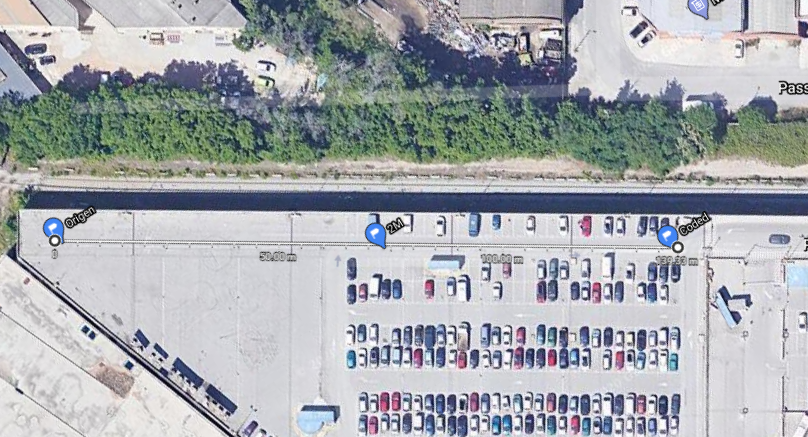
\includegraphics[width=\textwidth]{./images/prova_abast.png}
		\caption{Abast real de BLE}
		\label{abast}
	\end{center}
\end{figure}

El procediment per realitzar l'experiment va ser col·locar una de les PCB sobre un cotxe i amb l'altre connectada a un altre ordinador es va anar retrocedint fins que es perdés la connexió.
Per forçar que es perdés la connexió quan ja no es podia establir una comunicació des de la PCB que s'anava movent s'anaven enviant peticions de lectura d'atributs.

Els resultats obtinguts, que es poden veure en la Figura \ref{abast}, indiquen que la distància màxima d'abast del dispositiu en una capa 2M és de 75 metres, mentre que en una capa S=8 aquesta distància s'estén fins als 135 metres.
S'han tingut en compte únicament aquestes capes físiques, ja que com que no hi ha interferències significatives i sempre s'ha mantingut la visibilitat directa, els resultats de la capa 1M són similars als de 2M i els de Coded S=2 són similar als de S=8.
Així doncs, amb aquest experiment s'ha vist una de les millores de la capa física Coded, l'abast.
\newpage

També s'ha realitzat un mapa de cobertura de l'interior d'una casa per poder observar quin és l'abast en un escenari més habitual amb obstacles.
En aquest cas s'ha establert una connexió fins a la PCB i s'ha obtingut el valor de la potència rebuda en totes les estances de la casa. De les mesures preses s'ha realitzat un mapa de cobertura que es pot veure a la Figura \ref{heatmap}.

La PCB s'ha col·locat a l'habitació 1 i s'ha configurat amb la potència de transmissió de 0 dBm i amb la capa física LE 1M.
Just al costat de la PCB es reben -50 dBm i en l'altra punta de l'habitació hi ha -70 dBm, això es deu, als obstacles que hi ha entremig.
Al llarg del passadís la potència és de -62 dBm, és bona, ja que és la zona on hi ha visibilitat directa entre els dispositius.
A les estances adjuntes al passadís, el lavabo i l'habitació 2 la potència arriba a baixar fins a -80 dBm.

Més enllà a la cuina i al menjador es reben potències de -80 fins a -85 dBm.
Un cop passada la sala d'estar el senyal ja es veu greument afectada i es comencen a perdre alguns paquets. En aquesta estança es reben -90 dBm. A l'habitació 3, la connexió és molt pobre i és habitual que els dispositius perdin la connexió. En aquesta, la potència rebuda és d'entre -95 dBm i -100 dBm.
En el vestidor i el lavabo 2, que són les estances més allunyades de la casa, en travessar la porta sempre es perd la connexió.
Que es rebi connexió a l'habitació 3 i no al lavabo i vestidor del costat es deu al fet que el senyal penetra la paret i arriba més fàcilment.

Tal com es pot observar pel resultat, BLE pot aconseguir un abast considerable en interiors però no d'una punta a un altre de la casa.
En aquest escenari específic la configuració era adversa a propòsit per veure quin era el límit de la tecnologia.
En un cas més realista, hi hauria un repetidor (anb Mesh Profile) al centre de la casa que tindria una cobertura que abastaria qualsevol punt.
D'aquesta manera qualsevol sensor situat a les puntes de la casa tindria connectivitat sense problemes.
\newpage

\begin{figure}[!h]
	\begin{center}
		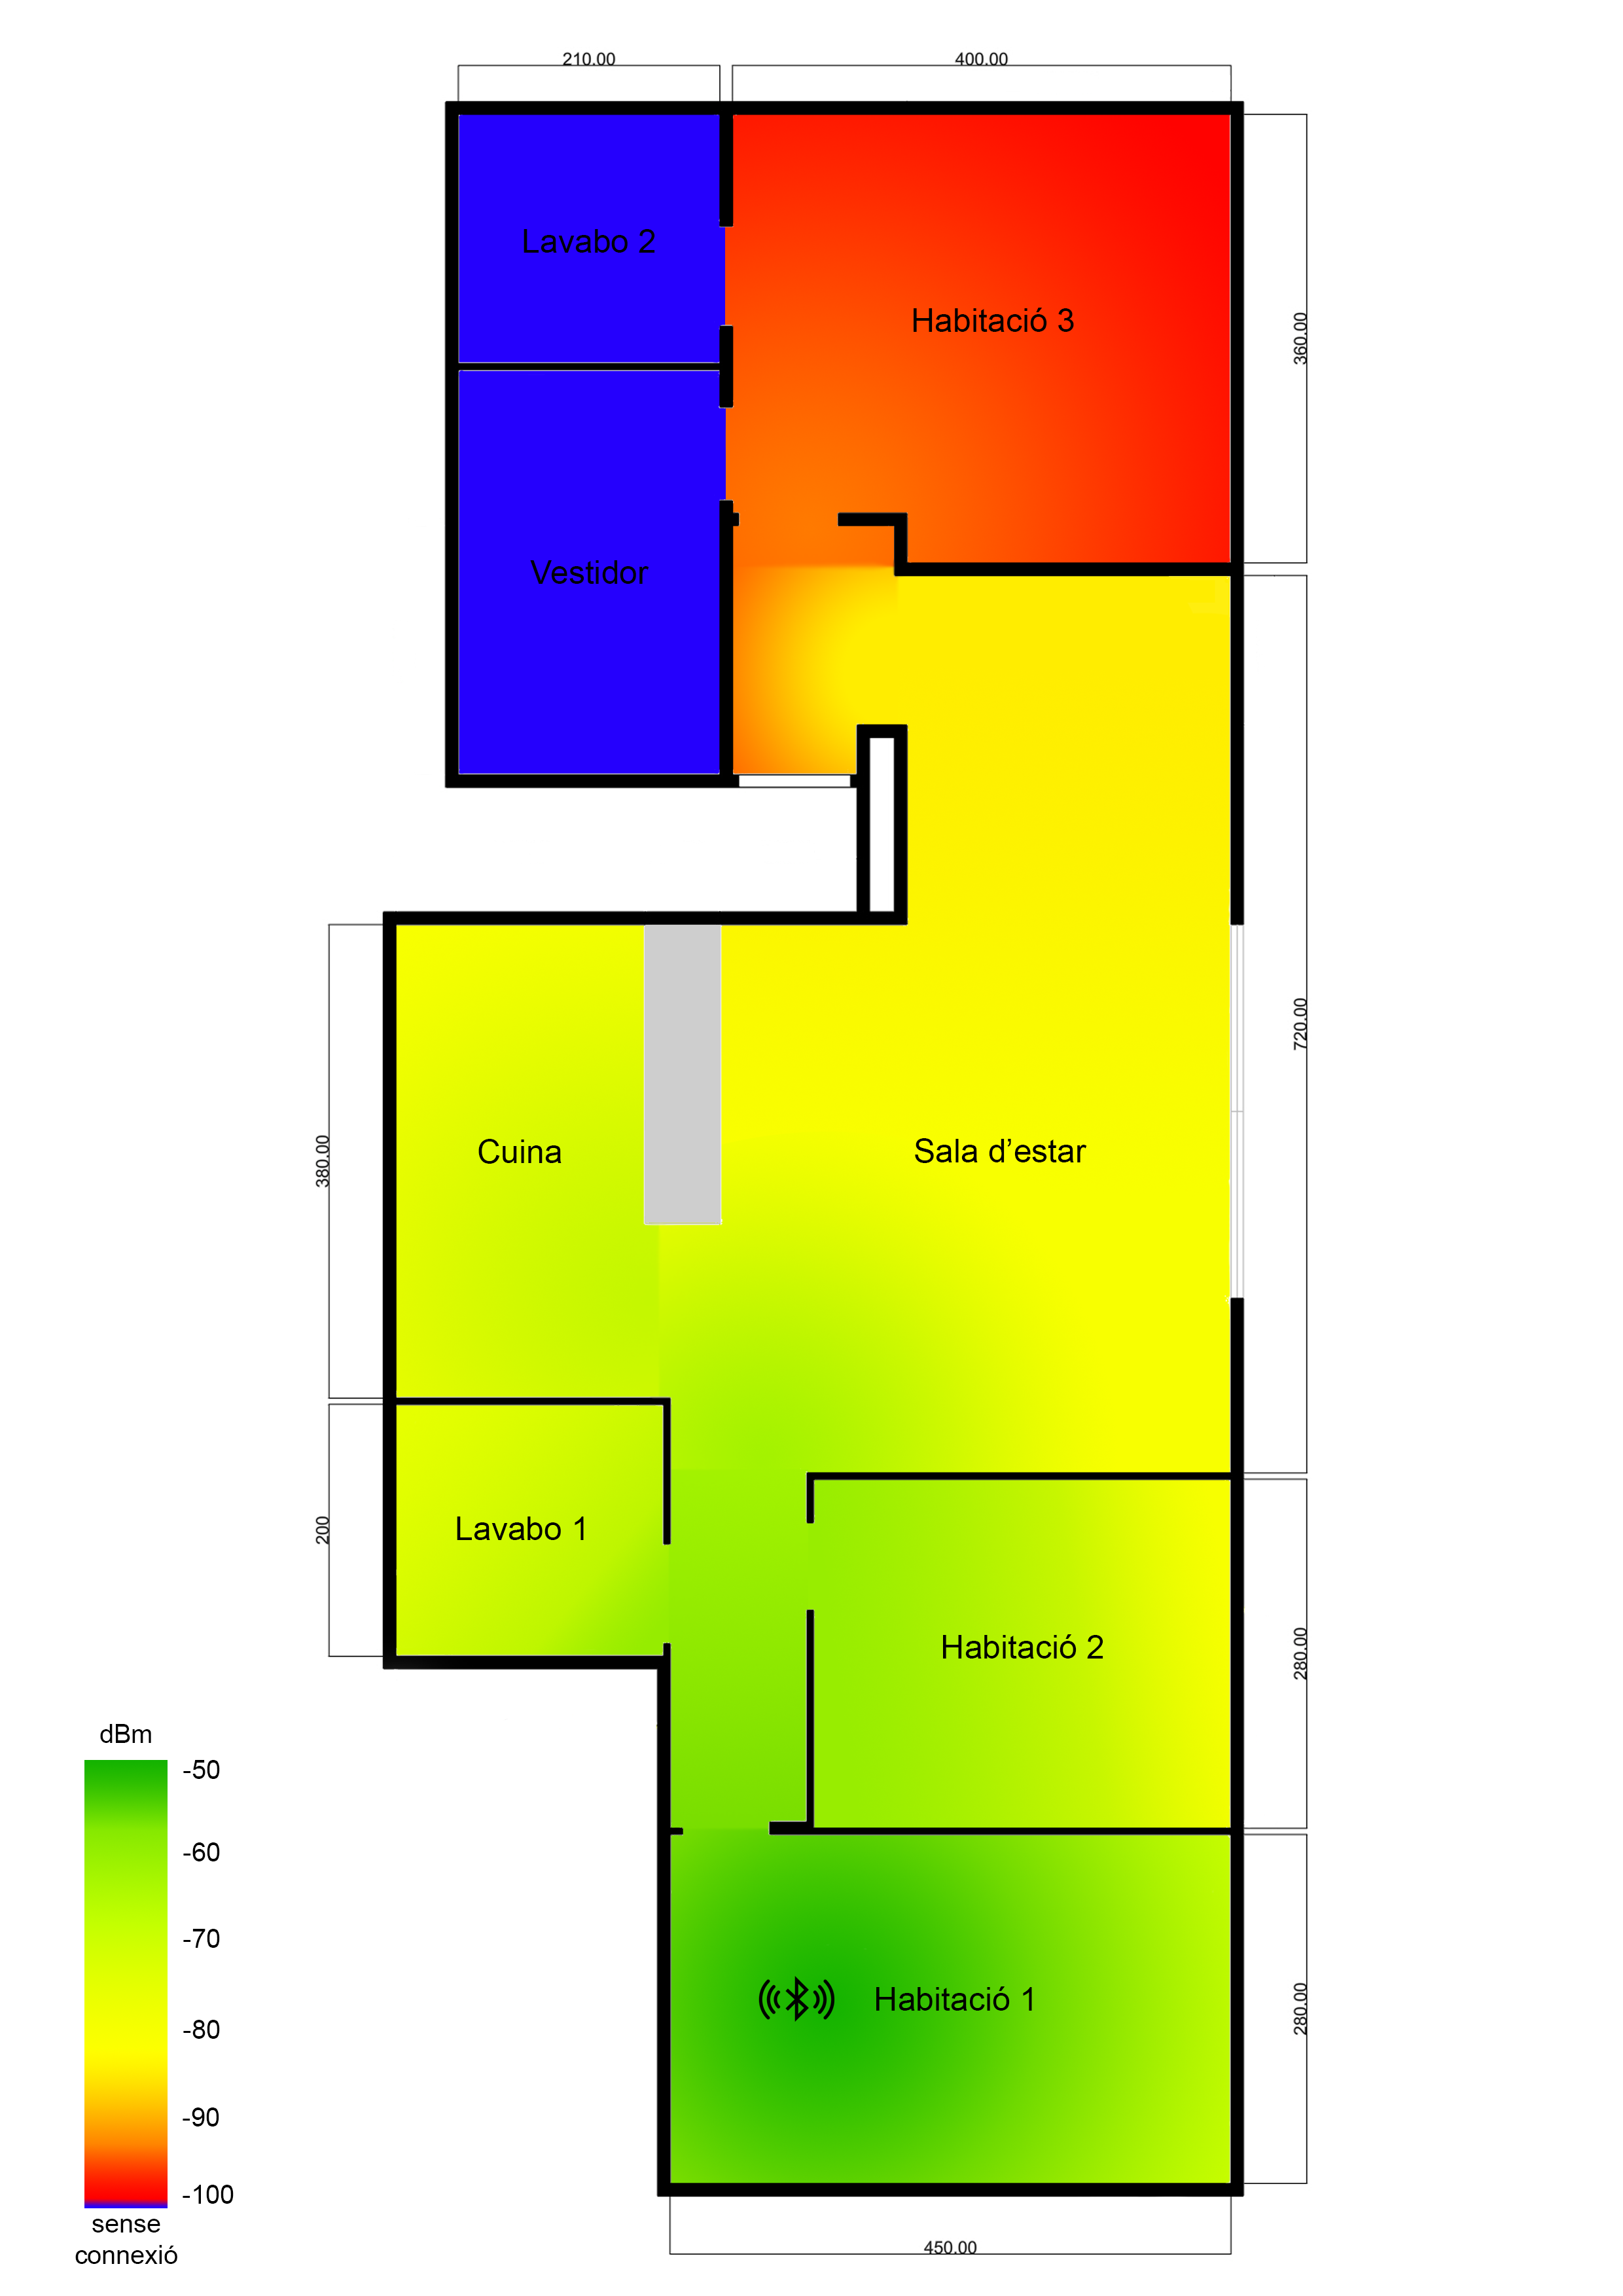
\includegraphics[width=\textwidth]{./images/hotmap.png}
		\caption{Mapa de cobertura}
		\label{heatmap}
	\end{center}
\end{figure}

\subsection{Consum d'energia}

El consum dels dispositius que utilitzen BLE és la característica més significativa, ja que, aquesta tecnologia està dissenyada per a consumir la menor quantitat d'energia possible.
Les PCB utilitzades tenen ponts extraïbles, tal com es pot veure en la Figura \ref{ponts_extraibles}, que permeten desconnectar els components que no són essencials per al funcionament del xip CC1352R.

\begin{figure}[h]
	\begin{center}
		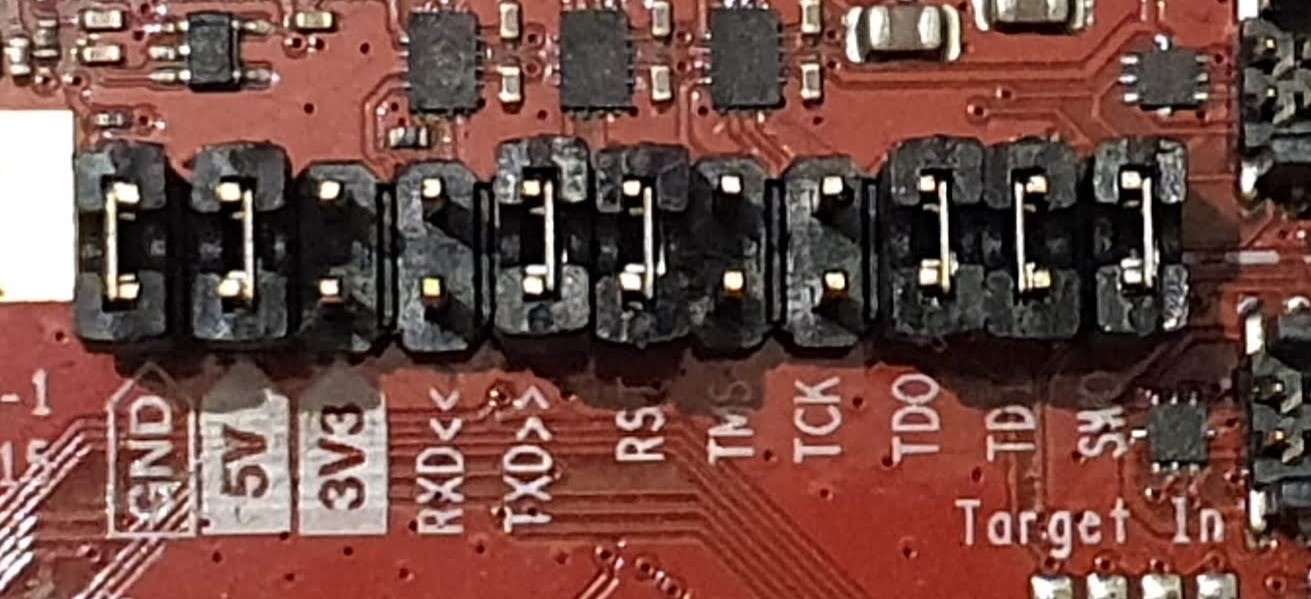
\includegraphics[width=0.7\textwidth]{./images/ponts.jpg}
		\caption{Ponts extraïbles de la PCB}
		\label{ponts_extraibles}
	\end{center}
\end{figure}

D'aquesta manera, es pot utilitzar un analitzador de potència per mesurar l'energia consumida.
Aquesta configuració produeix una mesura molt precisa i permet calcular el cicle de vida del dispositiu que s'està desenvolupant.
Per contra, no es poden utilitzar les eines de desenvolupament com la depuració del codi.

Per poder desenvolupar fàcilment un projecte i analitzar els canvis que el codi produeix en l'ús d'energia, existeix una eina anomenada Energy Trace.
D'aquesta manera, es pot analitzar comparativament en quin moment s'està consumint l'energia i es poden adaptar els paràmetres de la connexió per observar quin serà l'estalvi que s'aconseguirà.
És per això que, es poden prendre les decisions de quins sacrificis són assumibles, per exemple, augmentar la latència a canvi de reduir el consum.
Aquesta eina però, no substitueix la solució explicada anteriorment amb l'analitzador de potència, ja que l'Energy Trace resulta molt menys precisa.

Per provar el funcionament de l'Energy Trace s'ha utilitzat durant l'execució en el xip del Project Zero.
A la Figura \ref{energy_trace1} es pot observar una captura del consum aproximat de corrent del CC1352.

\begin{figure}[!h]
	\begin{center}
		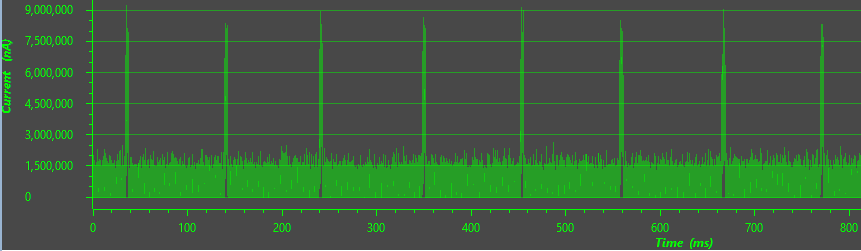
\includegraphics[width=\textwidth]{./images/consum_energia_no_connected_current2.png}
		\caption{Mesura de corrent sense connexió}
		\label{energy_trace1}
	\end{center}
\end{figure}

És possible visualitzar com hi ha pics de consum cada 100 ms, aquests corresponen als instants en què el dispositiu està enviant els anuncis.
Aquests 100 ms corresponen a l'interval d'anunci que s'ha configurat per a aquest projecte.

També és possible mesurar el consum d'energia acumulada de la PCB al llarg del temps, en aquest cas s'ha realitzat durant un segon i es pot veure a la Figura \ref{energy_measure}.

\begin{figure}[!h]
	\begin{center}
		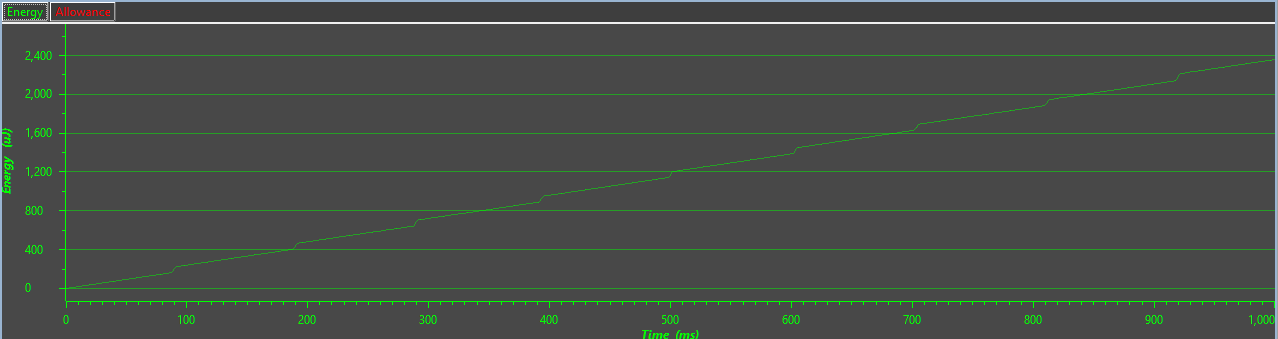
\includegraphics[width=\textwidth]{./images/consum_energia_no_connected_energia.PNG}
		\caption{Mesura d'energia sense connexió}
		\label{energy_measure}
	\end{center}
\end{figure}

Un cop s'estableix una connexió amb el dispositiu es realitza una altra captura del corrent que es pot observar a la Figura \ref{energy_trace_connection}.

\begin{figure}[!h]
	\begin{center}
		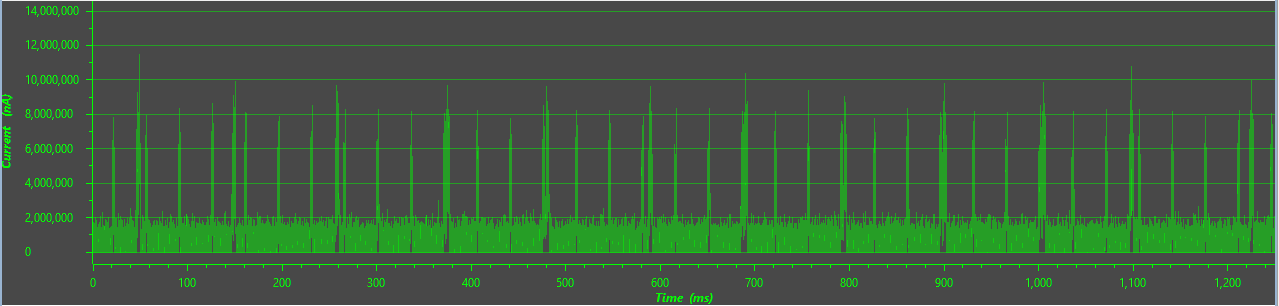
\includegraphics[width=\textwidth]{./images/consum_energia_connected_current.png}
		\caption{Mesura de corrent amb connexió}
		\label{energy_trace_connection}
	\end{center}
\end{figure}

A la gràfica és possible veure com segueixen estant els pics cada 100 ms però també n'hi ha cada 40 ms.
Aquests, darrers, es deuen als esdeveniments de connexió que en aquest cas estan configurats perquè es produeixen cada 40 ms.

En aquestes captures de consum de corrent, tot i que hi ha molta variació, es pot comprovar que mentre no es transmeten paquets, el consum és d'entre 0 i 2 mA.

També, es realitza una captura del consum d'energia acumulat durant un segon:

\begin{figure}[!h]
	\begin{center}
		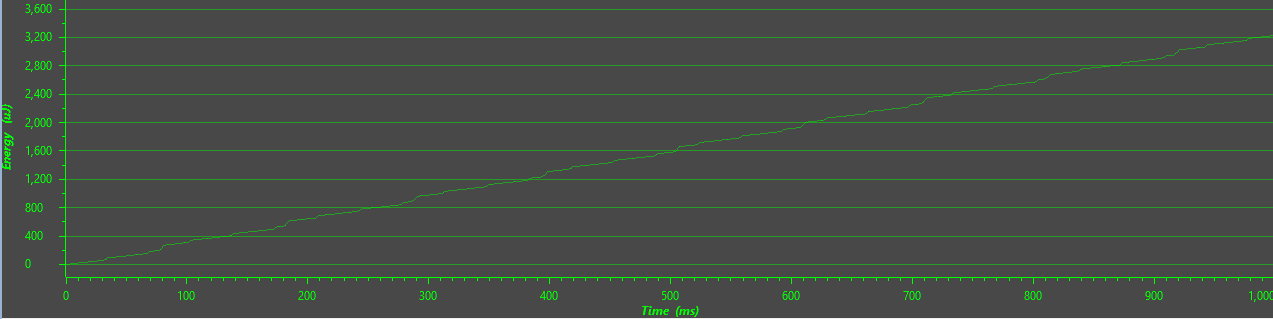
\includegraphics[width=\textwidth]{./images/consum_energia_connected_energy.png}
		\caption{Mesura d'energia amb connexió}
		\label{energy_trace2}
	\end{center}
\end{figure}

Els màxims que es produeixen per anuncis i per esdeveniments de connexió poden semblar similars en les captures de consum de corrent.
Tanmateix, no és així, en les captures de consum d'energia es pot observar com hi ha increments més pronunciats corresponents als anuncis i en canvi els esdeveniments de connexió els increments són més lleugers.

Si es veuen amb més detall l'anunci i l'esdeveniment (Figura \ref{energy_trace_adv} i Figura \ref{energy_trace_event}, respectivament) es pot observar com són d'una duració diferent.
D'una banda, l'anunci dura uns 4 mil·lisegons i mig, en canvi l'esdeveniment de connexió només dura 2 mil·lisegons.
\newline
\begin{figure}[!h]
	\begin{center}
		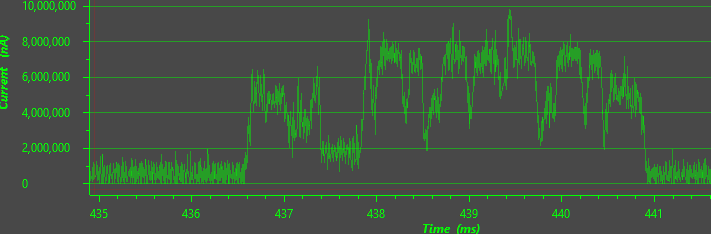
\includegraphics[width=\textwidth]{./images/pic_anunci_captura.png}
		\caption{Captura d'un anunci}
		\label{energy_trace_adv}
	\end{center}
\end{figure}
\begin{figure}[!h]
	\begin{center}
		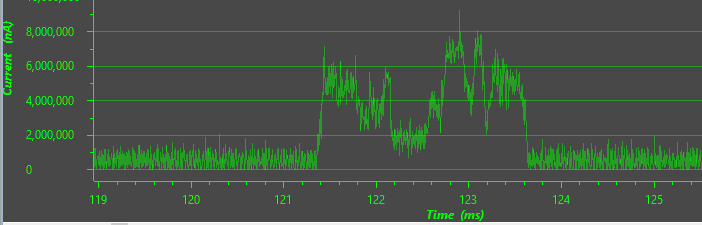
\includegraphics[width=\textwidth]{./images/pic_connectat_captura.png}
		\caption{Captura d'un esdeveniment}
		\label{energy_trace_event}
	\end{center}
\end{figure}

Aquesta eina, per tant, està orientada a facilitar una idea comparativa d'en quins instants es consumeix més energia.
D'aquesta manera, és més fàcil pel desenvolupador comprovar com els canvis en el codi afecten el consum d'energia.

A part dels gràfics, l'Energy Trace també proporciona directament les dades més rellevants de les captures.
A la Taula \ref{taula_consum} es troben els valors importants.\newline

\begin{table}[h!]
	\begin{center}
	\resizebox{\textwidth}{!}{%
		\renewcommand{\arraystretch}{2}
		\begin{tabular}{l|c|c|c|c|c|c|c|}
			\cline{2-8}
			\multirow{2}{*}{}                    & \multirow{2}{*}{\begin{tabular}[c]{@{}c@{}}Temps de Mesura\\ (s)\end{tabular}} & \multirow{2}{*}{\begin{tabular}[c]{@{}c@{}}Energia\\ (mJ)\end{tabular}} & \multicolumn{2}{c|}{Potència (mW)} & \multicolumn{2}{c|}{Corrent (mA)} & \multirow{2}{*}{Temps de Vida} \\ \cline{4-7}
			&                                                                                &                                                                         & mitjana          & màxim           & mitjana          & màxim          &                                \\ \hline
			\multicolumn{1}{|r|}{Sense Connexió} & 10                                                                             & 23,87                                                                   & 2,387            & 34,566          & 0,723            & 10,475         & 11 dies i 12 hores             \\ \hline
			\multicolumn{1}{|r|}{Amb Connexió}   & 10                                                                             & 32,57                                                                   & 3,257            & 41,672          & 0,987            & 12,63          & 8 dies i 10 hores              \\ \hline
		\end{tabular}%
		\renewcommand{\arraystretch}{1}
	}
	\end{center}
	\caption{Taula comparativa de mesures\label{taula_consum}}	
\end{table}

Per aquests valors s'han pres mesures de 10 segons de duració per obtenir unes mitjanes més representatives d'un ús continu.
Es pot observar com la potència i corrent màxim consumits, tant amb connexió com sense, no són molt diferents entre si.
Això es deu al fet que independentment de si el dispositiu té conexions establertes, s'enviaran els anuncis que suposen el pic més important de les gràfiques amb el consum de corrent.

Els paràmetres amb els quals s'ha pres la mesura no estan optimitzats específicament per a un consum molt baix, tot i això, es pot observar com en els dos casos la mitjana de consum és molt reduïda, per sota d'1 mA.
Per contextualitzar com és de baix aquest consum, és habitual calcular un temps de vida estimat d'una pila de botó, en aquest cas s'utilitza la CR2032.
En aquest cas, el temps de vida, tenint en compte la connexió seria de 8 dies.
Altrament, sense connexió aquest temps de vida s'allargaria fins als onze dies i mig.
Per tant, el temps de vida s'assimilarà més a 8 o 11 dies depenent del temps en què el dispositiu es passi amb alguna connexió.

Per contextualitzar-ho més, si s'utilitzés una bateria habitual en els telèfons mòbils que tingués 3800 mAh suposaria un temps de vida de 160 amb connexió i 219 dies sense, uns 7,3 i 5,3 mesos corresponentment.


\subsection{ADC}
L'\textit{Analogic to Digital Converter} és un perifèric de la PCB que permet convertir un senyal analògic a un digital.
Per poder comprovar que les capacitats de l'ADC de la PCB són suficients per a sensors s'ha realitzat un experiment.
Aquest es basa en comprovar que la PCB pot mostrejar prou ràpidament per mesurar els senyals que s'obtindrien dels sensors.

S'ha utilitzat un generador de funcions per simular un senyal d'ona quadrada i s'ha anat variant la freqüència del senyal. Aquest senyal s'ha connectat tant a l'oscil·loscopi com a la PCB utilitzant una T com es pot observar a la Figura \ref{lab}.

\begin{figure}[!h]
	\begin{center}
		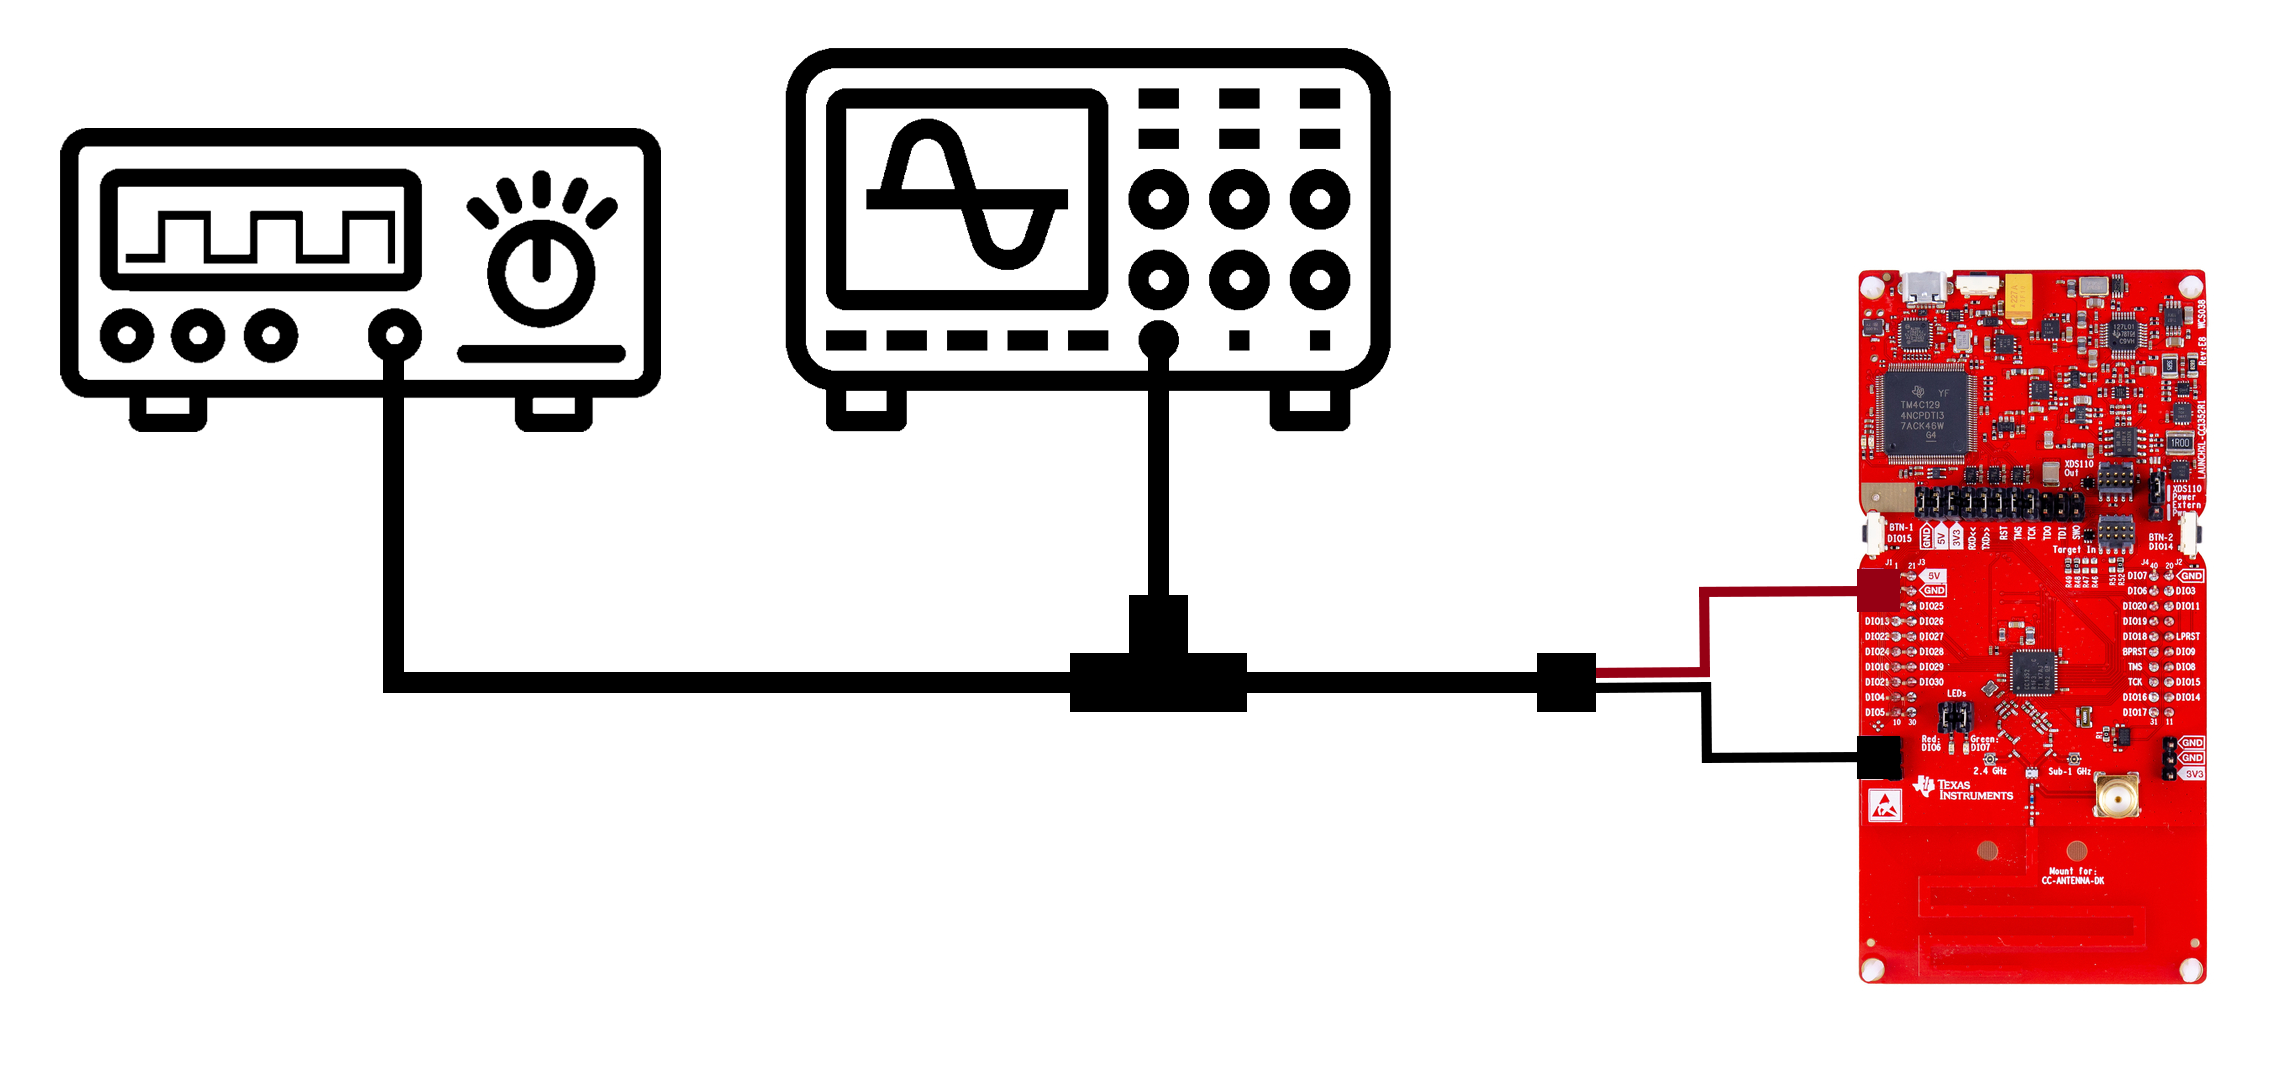
\includegraphics[width=0.9\textwidth]{./images/CicrcuitoExperimentoLab2.png}
		\caption{Escenari ADC \cite{icon_oscil}}
		\label{lab}
	\end{center}
\end{figure}


Com que l'ADC de la PCB té un rang de 0 a 3,3 V s'ha configurat el generador de funcions amb un òfset per tenir un senyal sempre en voltatge positiu.
L'amplitud del senyal és d'aproximadament 2,5 V, no és de 3,3 V perquè el generador de funcions sempre supera breument l'amplitud del senyal i d'aquesta manera s'evita superar els 3,3 V i protegir l'ADC.

En la PCB s'executarà el projecte \textit{adcBufContinous} que ve inclòs en els exemples del SimpleLink i permet realitzar mostres de l'ADC contínuament i les ensenya a través de la consola.
Originalment en aquest projecte es mostren els volts a l'entrada de l'ADC, però s'ha modificat perquè mostri zeros quan el voltatge està sota de 1,5 V i uns quan està per sobre de 1,5 V.
Sempre s'utilitza una freqüència de mostreig que sigui un múltiple de la freqüència del senyal i si s'està mostrejant correctament ha d'haver-hi el mateix nombre de mesures amb valor alt que amb baix.
Per tant, la consola ha de tenir una seqüència amb la mateixa quantitat de zeros que uns.

Per comprovar que s'està mostrejant el senyal correctament s'han mostrejat senyals amb una freqüència divisora de la freqüència de mostreig.
En aquest cas, si el senyal té la mateixa quantitat de zeros i uns i es repeteix cada $L$ mostres que vénen definides segons la Fòrmula \ref{eqn:length}, sent $f_{m}$ la freqüència de mostreig i $f_{s}$ la freqüència del senyal mostrejat.


\begin{equation}
	\label{eqn:length}
	L=\frac{f_{m}}{f_{s}}
\end{equation}

Primer de tot s'ha mostrejat a frequencies baixes per comprobar que els resultats fossin els esperats i per tant que l'escenari estigués ben implementat.

Amb una $f_{m}=20$Hz i una $f_{s}=10$Hz s'ha obtingut:
\begin{lstlisting}[language=C]
	Buffer: 0,1,0,1,0,1,0,1,0,1,0,1,0,1,0,1,0,1,0,1,
\end{lstlisting}

A continuació, s'ha configurat l'ADC per mostrejar a la màxima frequencia i s'han provat senyals amb frequencia divisora de la frequencia de mostreig.

Amb una $f_{m}=200$kHz i una $f_{s}=20$kHz s'ha obtingut:
\begin{lstlisting}[language=C]
	Buffer: 0,0,0,0,0,1,1,1,1,1,0,0,0,0,0,1,1,1,1,1,
\end{lstlisting}

Amb una $f_{m}=200$kHz i una $f_{s}=50$kHz s'ha obtingut:
\begin{lstlisting}[language=C]
	Buffer: 0,0,1,1,0,0,1,1,0,0,1,1,0,0,1,1,0,0,1,1,
\end{lstlisting}


Finalment s'ha provat amb el senyal a la màxima freqüència possible segons el teorema de Nyquist\footnote{El teorema de Nyquist defineix que si la freqüència de mostreig és el doble que la freqüència màxima d'un senyal, aquesta serà suficient per reconstruir el senyal mostrejat.}.

Amb una $f_{m}=200$kHz i una $f_{s}=100$kHz s'ha obtingut:
\begin{lstlisting}[language=C]
	Buffer: 0,1,0,1,0,1,0,1,0,1,0,1,0,1,0,1,0,1,0,1,
\end{lstlisting}

Tal com es pot observar, el senyal es continua mostrejant correctament i, per tant, es pot confirmar que és possible mostrejar senyals digitals de fins a 100 kHz.


També s'ha volgut comprovar si les mesures que pren l'ADC són precises.
S'han pres valors a diferents punts del rang dinàmic de l'ADC (0 - 3,3 V) tant amb l'ADC com amb un multímetre.
Amb aquestes mesures (que es poden trobar a l'Apèndix \ref{raw_adc}) s'ha realitzat un gràfic que es por veure a la Figura \ref{multimetre}.

\begin{figure}[!h]
	\begin{center}
		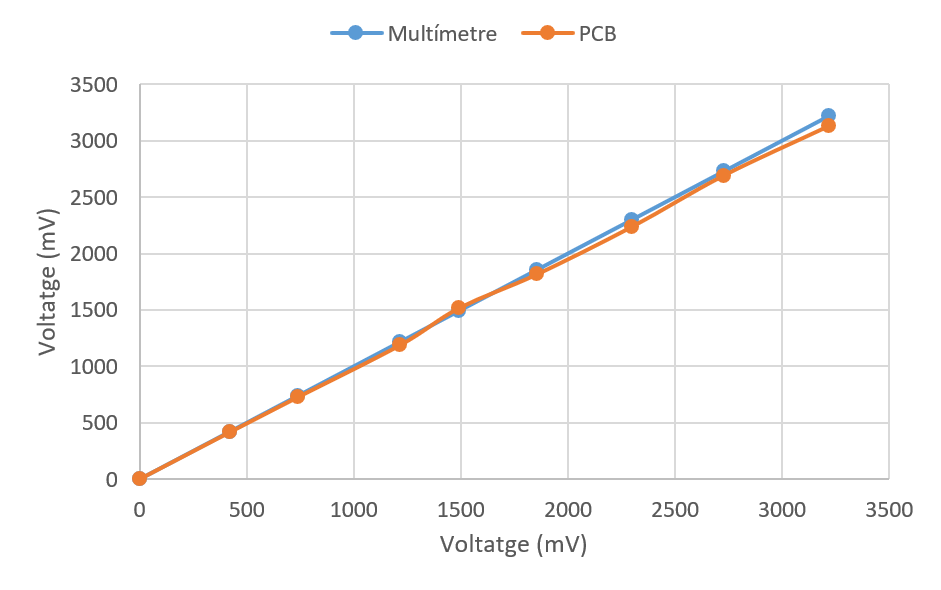
\includegraphics[width=0.8\textwidth]{./images/multimetre.PNG}
		\caption{Precisió ADC}
		\label{multimetre}
	\end{center}
\end{figure}

Com a referència s'han utilitzat les mesures del multímetre que formen la línia diagonal en blau.
La línia taronja mostra la mesura de l'ADC de la PCB i es pot veure com segueix de prop línia del multímetre.



\section{Lectura de l'ADC}
Per poder realitzar la lectura amb l'ADC, és necessari dissenyar un circuit per simular el senyal que produiria un sensor i també desenvolupar el codi necessari perquè la PCB prengui la mesura.
A continuació s'explicaran aquests processos.

\subsection{Disseny del simulador de sensors}
La PCB té un convertidor analògic-digital que ens permetrà enviar senyals analògics un cop s'han mostrejat.
En aquest treball no es tractaran directament els sensors sinó que es simularan els senyals que produirien.
Com que la PCB i el seu ADC treballen a 3,3$V$ es crearà un circuit que permeti controlar un voltatge d'entre 0 i 3,3$V$.

Aquest circuit es basarà en un divisor de voltatge simple format per una resistència i un potenciòmetre.
El potenciòmetre permet canviar la resistència de l'element a través d'un cargol i junt amb el circuit que l'envolta permetrà canviar el voltatge a la sortida.

\begin{figure}[!h]
	\begin{center}
		\begin{circuitikz}
			\draw
			(0,2) node[anchor=east] {$V_{in}$}
			to [R=$R_1$, *-] (2,2)
			to [vR=$R_{pot}$, *-] (2,0) node[tlground](GND){};
			\draw
			(2,2) to [short, -*] (3,2)
			to (3,2) node[anchor=west] (3,2) {$V_{out}$};
		\end{circuitikz}
		
	\end{center}
\end{figure}

Aquest circuit segueix l'estructura d'un divisor de voltatge per tant es pot calcular el voltatge a la sortida segons la següent fórmula.

\begin{equation}
	V_{in}\cdot\frac{R_{pot}}{R_1+R_{pot}}=V_{out}
\end{equation}

Per escollir els components cal tenir en compte utilitzar resistències de valor alt per reduir el consum d'energia.
S'utilitzarà un potenciòmetre de 10$k\Omega$ per tant serà una resistència que es podrà modificar des de 0$\Omega$ fins 10$k\Omega$.
Per trobar l'$R_1$ que compleixi els requisits queda la següent fórmula.

\begin{equation}
	R_1=5V\cdot\frac{10k\Omega}{3.3V}-10k\Omega\approx5151\Omega
\end{equation}

Per a l'$R_1$ s'utilitzaran resistències de la sèrie E12, els valors que més s'acosten a $5$,$121\Omega$ són $5.6k\Omega$ i $4.6k\Omega$.
Per assegurar-se que no es superen els 3.3$V$ a l'entrada de l'ADC que podria malmetre el dispositiu s'escull la resistència superior, per tant el circuit final queda dissenyat de la següent manera.

\begin{figure}[!h]
	\begin{center}
		\begin{circuitikz}
			\draw
			(0,2) node[anchor=east] {$5\,V$}
			to [R=$5.6\;k\Omega$, *-] (2,2)
			to [vR=$ \lbrack 0-10 \rbrack \;k\Omega$, *-] (2,0) node[tlground](GND){};
			\draw
			(2,2) to [short, -*] (3,2)
			to (3,2) node[anchor=west] (3,2) {$[0-3.3]\;V$};
		\end{circuitikz}
		
	\end{center}
\end{figure}

Com que s'utilitzaran 4 canals de l'ADC per mesurar, es necessiten 4 circuits com el que s'ha dissenyat.
S'ha implementat el circuit en una placa de proves i soldat els components de tal manera que cal connectar el voltatge d'entrada (a 5 $V$) en vermell, terra en negre i finalment quatre cables blaus on hi haurà el voltatge controlat pels quatre potenciòmetres.
Es pot veure el resultat a la Figura \ref{ports_placa}.


\subsection{Desenvolupament i implementació del codi}

Tal com s'ha comentat anteriorment la PCB que s'està utilitzant conté un ADC de vuit canals que s'utilitza per llegir valors de voltatge.

%Importar adcsinglechannel
En aquest exemple, l'objectiu és aconseguir la lectura dels valors del voltatge d'un pin de la PCB.
El següent codi permet fer una mesura del canal que s'indiqui a través de l'argument.
Inicialitza l'ADC de la PCB, pren le mesura i posteriorment retorna el resultat en mil·livolts.

\begin{lstlisting}[language=C]
static uint16_t takeMeasurement(uint_least8_t adcIndex){
	ADC_Handle adc;
	ADC_Params params;
	ADC_init();
	ADC_Params_init(&params);
	adc = ADC_open(adcIndex, &params);
	if (adc == NULL){
		Log_info0("ADC start Failed");
		while(1);
	}
	int_fast16_t res;
	uint16_t adcValue;
	res = ADC_convert(adc, &adcValue);
	
	if (res == ADC_STATUS_SUCCESS) {
		Log_info1("ADC result %d mV", adcValue);
	}
	else {
		Log_info0("ADC status failure");
	}
	ADC_close(adc);
	return adcValue;
}
\end{lstlisting}

Finalment, cal canviar el codi de BLE perquè quan es llegeixin els atributs es retorni el valor mesurat a l'ADC.
Per tant cal canviar la funció environmentalService\_ReadAttrCB tal com es veu a continuació.

\begin{lstlisting}[language=C]
  if(!memcmp(pAttr->type.uuid, temperatureUUID, pAttr->type.len))
{
	uint16_t adcValue = takeMeasurement(Board_ADC0);
	*pLen = (uint16_t)temperatureLen;
	memcpy(pValue, &adcValue, *pLen);
}
else if(!memcmp(pAttr->type.uuid, humidityUUID, pAttr->type.len))
{
	uint16_t adcValue = takeMeasurement(Board_ADC1);
	*pLen = (uint16_t)humidityLen;
	memcpy(pValue, &adcValue, *pLen);
}
\end{lstlisting}


\section{Aplicació mòbil}
Per veure un exemple simplificat d'un client que consumís els serveis oferits per la PCB, s'ha realitzat un desenvolupament propi d'una aplicació per a Android.
Aquesta aplicació llegeix contínuament els valors dels quatre atributs que té la PCB que corresponen amb els sensors.

Per poder interactuar amb la PCB el primer que cal és tenir en compte l'adreça del dispositiu i els identificadors, tant del servei, com dels atributs.
Aquests es poden veure a la Taula \ref{taula_app}

\begin{table}[!h]
	\begin{center}
		\begin{tabular}{|c|l|}
			\hline
			Identificador	&	Valor	\\	\hline
			deviceAddress	&	00:81:F9:4A:4D:B3	\\	\hline
			serviceUUID		&	f0001234-0451-4000-b000-00000000		\\	\hline
			temperatureUUID	&	f0002345-0451-4000-b000-000000000000	\\	\hline
			humidityUUID	&	f0003456-0451-4000-b000-000000000000	\\	\hline
			heartRateUUID	&	f0004567-0451-4000-b000-000000000000	\\	\hline
			bloodOxygenUUID	&	f0005678-0451-4000-b000-000000000000	\\	\hline
		\end{tabular}
		\label{taula_app}
	\end{center}
	\caption{Tipus d'anunciaments}
\end{table}

Per realitzar l'aplicació d'Android cal declarar que requereix els permisos de Bluetooth i específicament de Bluetooth Low Energy.

\begin{lstlisting}[language=xml]
	<uses-permission android:name="android.permission.BLUETOOTH"/>
	<uses-feature android:name="android.hardware.bluetooth_le" android:required="true"/>
\end{lstlisting}

Per implementar el BLE en Android s'ha utilitzat la llibreria nativa que es pot trobar a \cite{ble_library} i s'ha seguit la guia que es troba a \cite{ble_overview}.

Primerament, per poder utilitzar BLE, s'inicialitza l'adaptador corresponent.

\begin{lstlisting}[language=java]
final BluetoothManager bluetoothManager =
	(BluetoothManager) getSystemService(Context.BLUETOOTH_SERVICE);
BluetoothAdapter bluetoothAdapter = bluetoothManager.getAdapter();
\end{lstlisting}

A continuació es comença a escanejar per buscar dispositius.
Per fer-ho es defineix una funció de \textit{callback} que filtrarà els dispositius per comprovar que es troba el que es vol.

\begin{lstlisting}[language=java]
bluetoothLeScanner.startScan(leScanCallback);
\end{lstlisting}

La funció leScanCallback quan trobi el dispositiu al qual vol connectar-se, deixarà d'escanejar i procedirà a intentar connectar-s'hi.
\begin{lstlisting}[language=java]
if(result.getDevice().getAddress().equals(deviceAddress)){
	bluetoothLeScanner.stopScan(leScanCallback);
	device = result.getDevice();
	bluetoothGatt = device.connectGatt(getApplicationContext(), false, gattCallback);
}
\end{lstlisting}

A l'establir la connexió es descobreixen els serveis del dispositiu.
S'obté el servei específic que volem i es llegeixen les característiques corresponents.

\begin{lstlisting}[language=java]
BluetoothGattService service = gatt.getService(
	UUID.fromString(serviceUUID));
characteristicList = service.getCharacteristics();
readCharacteristic(gatt);
\end{lstlisting}

Per cada característica que es llegeix, per obtenir el seu valor tal com es vol mostrar i no com l'envia BLE (en little-endian), cal especificar el format que té.
En aquest cas, com que s'han definit en 2 bytes les longituds de les característiques en la PCB, cal especificar que són nombres enters \textit{unsigned} (sense signe) codificats en 16 bits.

\begin{lstlisting}[language=java]
int characteristicValue = characteristic.getIntValue(
BluetoothGattCharacteristic.FORMAT_UINT16, 0);
\end{lstlisting}

Les dades que s'estan transmetent per cada atribut corresponen al valor del voltatge.
Tot i això, per caracteritzar aquestes dades a l'aplicació s'interpreten com si fossin valors plausibles de les mesures que s'estan prenent.
Igualment, es mostra tant una barra de progrés com el valor real de mil·livolts per cada mesura de la PCB.
Però per poder mostrar aquests valors no es pot fer directament.
El codi de BLE és asíncron i es troba en un fil d'execució (\textit{thread} en anglès) diferent al que controla la interfície d'usuari.
Per poder compartir valors entre threads cal utilitzar un \textit{handler}.

Per passar múltiples valors amb un \textit{handler} cal fer-ho utilitzant \textit{bundles} tal com mostra el codi següent.
\begin{lstlisting}[language=java]
Bundle bundle = new Bundle();
bundle.putString("value", Integer.toString(characteristicValue));
bundle.putString("characteristic",characteristic.getUuid().toString());
Message message = new Message();
message.obj = bundle;
updateHandler.sendMessage(message);
\end{lstlisting}

Aquests valors es reben a una funció que ja sí que pot modificar la interfície d'usuari i s'obtenen tal i es mostra en el codi a continuació.

\begin{lstlisting}[language=java]
 Handler updateHandler = new Handler(){
	@Override
	public void handleMessage(@NonNull Message msg) {
		super.handleMessage(msg);
		Bundle data = (Bundle) msg.obj;
		String characteristic = data.getString("characteristic");
		String value = data.getString("value");
		...
	}
}
\end{lstlisting}

Abans de modificar la interfície cal adaptar els valors que es reben per mostrar-los representant els sensors que s'han simulat.
Es suposa que els valors rebuts estaran entre 0 i 3000 que són els milivolts que ha llegit l'ADC de la PCB.
Cada mesura es caracteritza diferent, a continuació es pot observar el cas de la temperatura.

\begin{lstlisting}[language=java]
 switch (characteristic) {
	case temperatureUUID: {
		int val = Integer.parseInt(value);
		int progress = val * 30 / 3000;
		TextView tmpConverted =findViewById(R.id.temperatureConverted_lbl);
		TextView temperatureRaw = findViewById(R.id.temperatureRaw_lbl);
		ProgressBar pb = findViewById(R.id.temperature_pb);
		tmpConverted.setText(progress + "C");
		temperatureRaw.setText(value + "mV");
		pb.setProgress(progress);
		break;
	}
\end{lstlisting}

En aquest cas, la temperatura s'assumeix que tindrà valors des de 0 fins a 30 graus.
Finalment, es calcula el seu valor en graus i es canvia la interfície perquè representi el valor.
El codi complet de l'aplicació que s'ha realitzat es pot trobar a \cite{android_repo}.

\newpage
\section{Escenari}
Finalment, un cop desenvolupat el circuit per simular sensors, el codi necessari per mostrejar i transmetre els valors i una aplicació per rebre aquests valors, l'escenari és el següent.

El circuit que simula els 4 sensors es connecta als pins de la PCB (veure Apèndix \ref{datasheet}) que tenen ADC segons el manual de la PCB que es pot trobar a \cite{manual_placa} seguint la Taula \ref{connexions}.

\begin{table}[!h]
	\begin{center}
		\begin{tabular}{|c|c|c|}
			\hline
			ADC			&	DIO		& 	PIN		\\	\hline
			0			&	23		&	2		\\	\hline
			1			&	24		&	6		\\	\hline
			2			&	25		&	23		\\	\hline
			3			&	26		&	24		\\	\hline
		\end{tabular}
	\end{center}
	\caption{Taula dels pins amb ADC}
	\label{connexions}
\end{table}

Les connexions des del circuit fins a la PCB es fan a través dels ports que proporciona la PCB a la seva part de darrere que es veuen a la Figura \ref{ports_placa}.

\begin{figure}[h]
	\begin{center}
		\includegraphics[width=\textwidth]{./images/PlacaUnion2.png}
		\caption{Ports de la PCB}
		\label{ports_placa}
	\end{center}
\end{figure}

Un cop fetes les connexions, cal executar el codi de la PCB i clicar el botó d'escanejar de l'aplicació.
Cal tenir en compte que durant el procés d'escaneig, degut a la configuració de BLE, sempre és possible (tot i que poc probable) que el mòbil no descobreixi la PCB un cop transcorregut el temps establert.
En aquest cas, cal tornar a clicar el botó d'escaneig.
Un cop l'aplicació està escanejant es poden canviar les posicions dels potenciòmetres i s'observa com els valors corresponents en el mòbil canvien amb poca latència.
Es pot veure una captura del disseny de l'aplicació a la Figura \ref{captura_app}.

\begin{figure}[h!]
	\begin{center}
		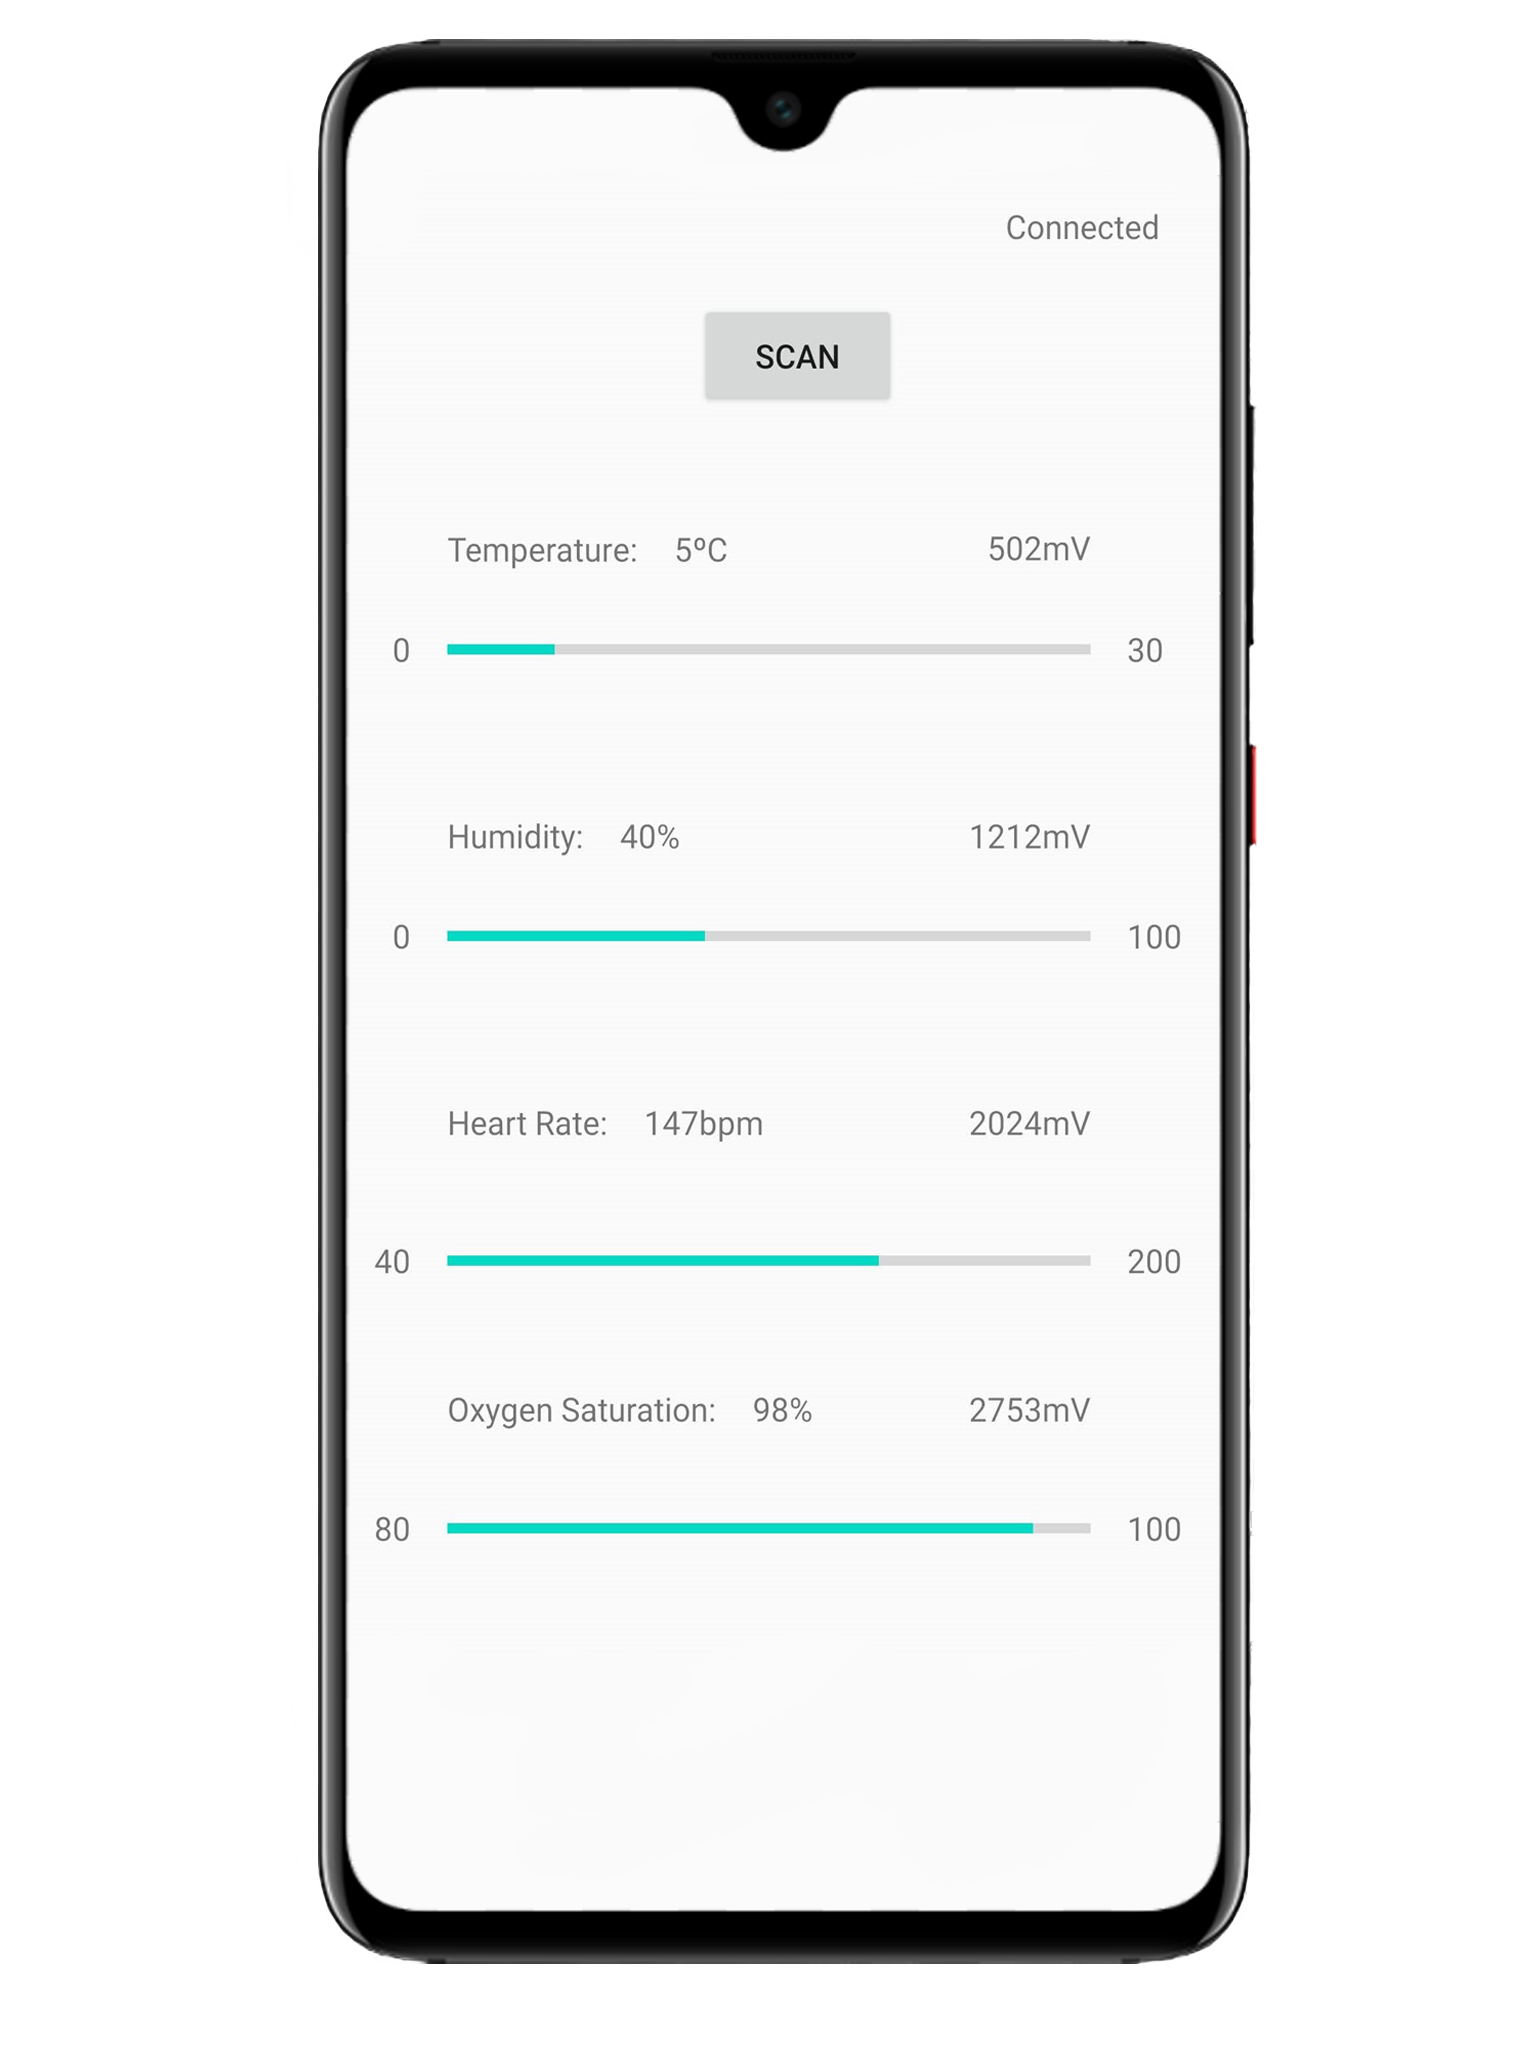
\includegraphics[width=0.6\textwidth]{./images/captura_app_borde.png}
		\caption{Aplicació mòbil}
		\label{captura_app}
	\end{center}
\end{figure}

\newpage
\section{Continuïtat del projecte}
Un cop executat el projecte i entès tant la tecnologia Bluetooth Low Energy com l'entorn de desenvolupament, hi ha aspectes en els quals és possible profunditzar més.
Aquestes es podrien tractar en un altre futur treball.

Tal com s'ha esmentat quan s'ha realitzat l'estudi del consum d'energia utilitzant Energy Trace, els valors obtinguts no es poden considerar absoluts.
És per això que, per poder determinar el temps de vida amb molta més precisió amb diferents configuracions del BLE s'hauria de mesurar el consum amb un oscil·loscopi mentre la PCB està configurada amb la font d'alimentació externa.

La implementació pràctica de BLE que s'ha realitzat utilitza únicament serveis propis.
Seria interessant implementar un servei estandarditzat i tenir algun dispositiu comercial que pogués connectar-se a la PCB.

Finalment, tot i haver-se desenvolupats projectes que permeten mesurar els voltatges dels ADC i emetre notificacions, per part de BLE, no s'ha aconseguit que sigui alhora.

